
%{{第二十一回}}{第二十一回}}

\chapter[贤袭人娇嗔箴宝玉 俏平儿软语救贾琏]{\texorpdfstring{贤袭人{\protect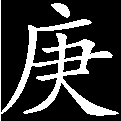
\includegraphics[width=3mm]{../Images/00004}\protect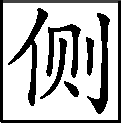
\includegraphics[width=3mm]{../Images/00011}\footnotesize \kaishu 当得起。}娇嗔箴宝玉 俏平儿软语救贾琏}{贤袭人庚辰本侧批当得起。娇嗔箴宝玉 俏平儿软语救贾琏}}
{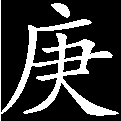
\includegraphics[width=3mm]{../Images/00004}有客题《红楼梦》一律,失其姓氏,惟见其诗意骇警,故录于斯:}

{    自执金矛又执戈,自相戕戮自张罗。}

{    茜纱公子情无限,脂砚先生恨几多。}

{    是幻是真空历遍,闲风闲月枉吟哦。}

{    情机转得情天破,情不情兮奈我何?}

{凡是书题者,不可{[}不以{]}此为绝调。诗句警拔,且深知拟书底里,惜乎失名矣!按此回之文固妙,然未见后之卅回,犹不见此之妙。此曰``娇嗔箴宝玉''、``软语救贾琏'',后曰``薛宝钗借词含讽谏,王熙凤知命强英雄''。今只从二婢说起,后则直指其主。然今日之袭人、之宝玉,亦他日之袭人、他日之宝玉也。今日之平儿、之贾琏,亦他日之平儿、他日之贾琏也。何今日之玉犹可箴,他日之玉已不可箴耶?今日之琏犹可救,他日之琏已不可救耶?箴与谏无异也,而袭人安在哉?宁不悲乎!救与强无别也,甚矣,今因平儿救,此日阿凤英气何如是也?他日之强,何身微运蹇,展眼何如彼耶?人世之变迁如此,光阴倏尔如此!}

{今日写袭人,后文写宝钗;今日写平儿,后文写阿凤。文是一样情理,景况光阴,事却天壤矣!多少恨泪洒出此两回书。}

{此回袭人三大功,直与宝玉一生三大病映射。}

话说史湘云跑了出来,怕林黛玉赶上,宝玉在后忙说:``仔细绊跌了!那里就赶上了?''林黛玉赶到门前,被宝玉叉手在门框上拦住,笑劝道:``饶他这一遭罢。''林黛玉搬着手说道:``我若饶过云儿,再不活着!''湘云见宝玉拦住门,料黛玉不能出来,{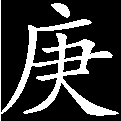
\includegraphics[width=3mm]{../Images/00004}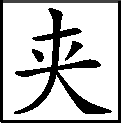
\includegraphics[width=3mm]{../Images/00012}\footnotesize \kaishu 写得湘云与宝玉又亲厚之极,却不见疏远黛玉,是何情思耶?}便立住脚笑道:``好姐姐,饶我这一遭罢。''恰值宝钗来在湘云身后,也笑道:``我劝你两个看宝兄弟分上,都丢开手罢。''{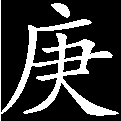
\includegraphics[width=3mm]{../Images/00004}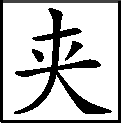
\includegraphics[width=3mm]{../Images/00012}\footnotesize \kaishu 好极,妙极!玉、颦、云三人已难解难分,插入宝钗云``我劝你两个看宝玉兄弟分上'',话只一句,便将四人一齐笼住,不知孰远孰近,孰亲孰疏,真好文字!}黛玉道:``我不依。你们是一气的,都戏弄我不成!''{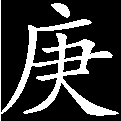
\includegraphics[width=3mm]{../Images/00004}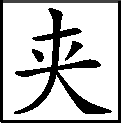
\includegraphics[width=3mm]{../Images/00012}\footnotesize \kaishu 话是颦儿口吻,虽属尖利,真实堪爱堪怜。}宝玉劝道:``谁敢打趣你!你不打趣他,他焉敢说你?''{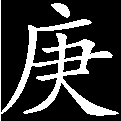
\includegraphics[width=3mm]{../Images/00004}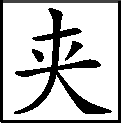
\includegraphics[width=3mm]{../Images/00012}\footnotesize \kaishu 好!二``你''字连二``他''字,华灼之至!}四人正难分解,{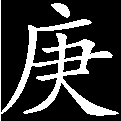
\includegraphics[width=3mm]{../Images/00004}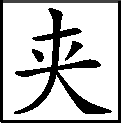
\includegraphics[width=3mm]{../Images/00012}\footnotesize \kaishu 好!前三人,今忽四人,俱是书中正眼,不可少矣。}有人来请吃饭,方往前边来。{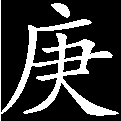
\includegraphics[width=3mm]{../Images/00004}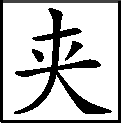
\includegraphics[width=3mm]{../Images/00012}\footnotesize \kaishu 好文章!正是闺中女儿口角之事。若只管谆谆不已,则成何文矣!}那天早又掌灯时分,王夫人、李纨、凤姐、迎、探、惜等都往贾母这边来,大家闲话了一回,各自归寝。湘云仍往黛玉房中安歇。{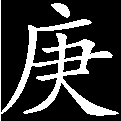
\includegraphics[width=3mm]{../Images/00004}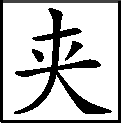
\includegraphics[width=3mm]{../Images/00012}\footnotesize \kaishu 前文黛玉未来时,湘云、宝玉则随贾母。今湘云已去,黛玉既来,年岁渐成,宝玉各自有房,黛玉亦各有房,故湘云自应同黛玉一处也。}

宝玉送他二人到房,那天已二更多时,袭人来催了几次,方回自己房中来睡。次日天明时,便披衣靸鞋往黛玉房中来,不见紫鹃、翠缕二人,只见他姊妹两个尚卧在衾内。那林黛玉{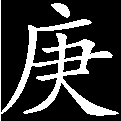
\includegraphics[width=3mm]{../Images/00004}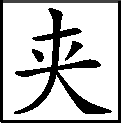
\includegraphics[width=3mm]{../Images/00012}\footnotesize \kaishu 写黛玉身分。}严严密密裹着一幅杏子红绫被,安稳合目而睡。{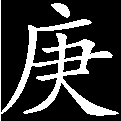
\includegraphics[width=3mm]{../Images/00004}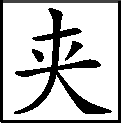
\includegraphics[width=3mm]{../Images/00012}\footnotesize \kaishu 一个睡态。}那史湘云却一把青丝拖于枕畔,被只齐胸,一弯雪白的膀子掠于被外,又带着两个金镯子。{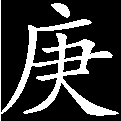
\includegraphics[width=3mm]{../Images/00004}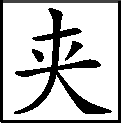
\includegraphics[width=3mm]{../Images/00012}\footnotesize \kaishu 又一个睡态。写黛玉之睡态,俨然就是娇弱女子,可怜。湘云之态,则俨然是个娇态女儿,可爱。真是人人俱尽,个个活跳,吾不知作者胸中埋伏多少裙钗。}宝玉见了,叹道:{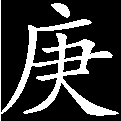
\includegraphics[width=3mm]{../Images/00004}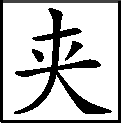
\includegraphics[width=3mm]{../Images/00012}\footnotesize \kaishu ``叹''字奇!除玉卿外,世人见之自曰喜也。}``睡觉还是不老实!回来风吹了,又嚷肩窝疼了。''一面说,一面轻轻的替他盖上。林黛玉早已醒了,{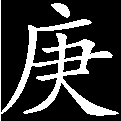
\includegraphics[width=3mm]{../Images/00004}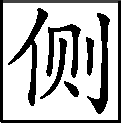
\includegraphics[width=3mm]{../Images/00011}\footnotesize \kaishu 不醒不是黛玉了。}觉得有人,就猜着定是宝玉,因翻身一看,果中其料。因说道:``这早晚就跑过来作什么?''宝玉笑道:``这天还早呢!你起来瞧瞧。''黛玉道:``你先出去,让我们起来。''{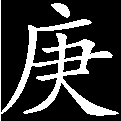
\includegraphics[width=3mm]{../Images/00004}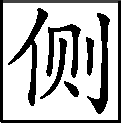
\includegraphics[width=3mm]{../Images/00011}\footnotesize \kaishu 一丝不乱。}宝玉听了,转身出至外边。

黛玉起来叫醒湘云,二人都穿了衣服。宝玉复又进来,坐在镜台旁边,只见紫鹃、雪雁进来伏侍梳洗。湘云洗了面,翠缕便拿残水要泼,宝玉道:``站着,我趁势洗了就完了,省得又过去费事。''说着便走过来,弯腰洗了两把。{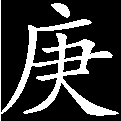
\includegraphics[width=3mm]{../Images/00004}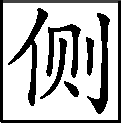
\includegraphics[width=3mm]{../Images/00011}\footnotesize \kaishu 妙在``两把''。}紫鹃递过香皂去,宝玉道:``这盆里的就不少,不用搓了。''{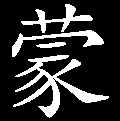
\includegraphics[width=3mm]{../Images/00006}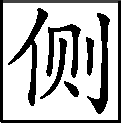
\includegraphics[width=3mm]{../Images/00011}\footnotesize \kaishu 此等用心淫极,请看却自不淫,非世之凡夫俗子得梦见者,真雅极趣极。}再洗了两把,便要手巾。{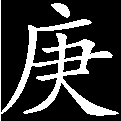
\includegraphics[width=3mm]{../Images/00004}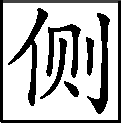
\includegraphics[width=3mm]{../Images/00011}\footnotesize \kaishu 在怡红何其费事多多。}翠缕道:``还是这个毛病儿,多早晚才改。''{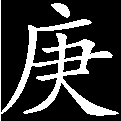
\includegraphics[width=3mm]{../Images/00004}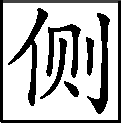
\includegraphics[width=3mm]{../Images/00011}\footnotesize \kaishu 冷眼人旁点,一丝不漏。}宝玉也不理,忙忙的要过青盐擦了牙,漱了口,完毕,见湘云已梳完了头,便走过来笑道:``好妹妹,替我梳上头罢。''湘云道:``这可不能了。''宝玉笑道:``好妹妹,你先时怎么替我梳了呢?''湘云道:``如今我忘了,{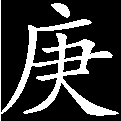
\includegraphics[width=3mm]{../Images/00004}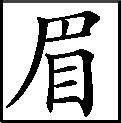
\includegraphics[width=3mm]{../Images/00010}\footnotesize \kaishu ``忘了''二字在娇憨口中自是应声而出,捉笔人却从何处设想而来,成此天然对答。壬午九月。}怎么梳呢?''宝玉道:``横竖我不出门,又不带冠子勒子,不过打几根散辫子就完了。''说着,又千妹妹万妹妹的央告。{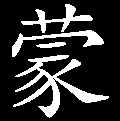
\includegraphics[width=3mm]{../Images/00006}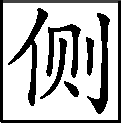
\includegraphics[width=3mm]{../Images/00011}\footnotesize \kaishu 逼近情态。}湘云只得扶他的头过来,一一梳篦。在家不戴冠,并不总角,只将四围短发编成小辫,往顶心发上归了总,编一根大辫,红绦结住。自发顶至辫梢,一路四颗珍珠,下面有金坠脚。湘云一面编着,一面说道:``这珠子只三颗了,这一颗不是的。{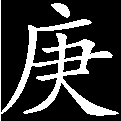
\includegraphics[width=3mm]{../Images/00004}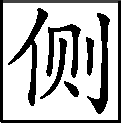
\includegraphics[width=3mm]{../Images/00011}\footnotesize \kaishu 梳头亦有文字,前已叙过,今将珠子一穿插,却天生有是事。}我记得是一样的,怎么少了一颗?''宝玉道:``丢了一颗。''湘云道:``必定是外头去掉下来,不防被人拣了去,倒便宜他。''{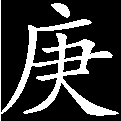
\includegraphics[width=3mm]{../Images/00004}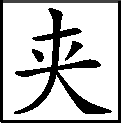
\includegraphics[width=3mm]{../Images/00012}\footnotesize \kaishu 妙谈!``倒便宜他''四字,是大家千金口吻。近日多用``可惜了的''四字。今失一珠,不闻此四字。妙极!是极!{ 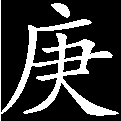
\includegraphics[width=3mm]{../Images/00004}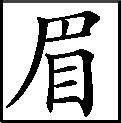
\includegraphics[width=3mm]{../Images/00010}\footnotesize \kaishu ``倒便宜他''四字与``忘了''二字是一气而来,将一侯府千金白描矣。畸笏。 }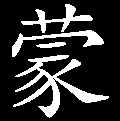
\includegraphics[width=3mm]{../Images/00006}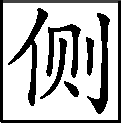
\includegraphics[width=3mm]{../Images/00011}\footnotesize \kaishu 是湘云口气。}黛玉一旁盥手,冷笑道:{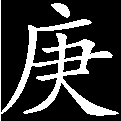
\includegraphics[width=3mm]{../Images/00004}\includegraphics[width=3mm]{../Images/00011}\footnotesize \kaishu 纯用画家烘染法。}``也不知是真丢了,也不知是给了人镶什么戴去了!''{\includegraphics[width=3mm]{../Images/00006}\includegraphics[width=3mm]{../Images/00011}\footnotesize \kaishu 是黛玉口气。}宝玉不答,{\includegraphics[width=3mm]{../Images/00004}\includegraphics[width=3mm]{../Images/00012}\footnotesize \kaishu 有神理,有文章。}因镜台两边俱是妆奁等物,顺手拿起来赏玩,{\includegraphics[width=3mm]{../Images/00004}\includegraphics[width=3mm]{../Images/00012}\footnotesize \kaishu 何赏玩也?写来奇特。}不觉又顺手拈了胭脂,意欲要往口边送,{\includegraphics[width=3mm]{../Images/00004}\includegraphics[width=3mm]{../Images/00012}\footnotesize \kaishu 是袭人劝后馀文。}因又怕史湘云说。{\includegraphics[width=3mm]{../Images/00004}\includegraphics[width=3mm]{../Images/00012}\footnotesize \kaishu 好极!的是宝玉也。}正犹豫间,湘云果在身后看见,一手掠着辫子,便伸手来``拍''的一下,从手中将胭脂打落,说道:``这不长进的毛病儿,多早晚才改过!''{\includegraphics[width=3mm]{../Images/00004}\includegraphics[width=3mm]{../Images/00011}\footnotesize \kaishu 前翠缕之言并非白写。}

一语未了,只见袭人进来,看见这般光景,知是梳洗过了,只得回来自己梳洗。忽见宝钗走来,因问道:``宝兄弟那去了?''袭人含笑道:``宝兄弟那里还有在家的工夫!''宝钗听说,心中明白。又听袭人叹道:``姊妹们和气,也有个分寸礼节,也没个黑家白日闹的!凭人怎么劝,都是耳旁风。''宝钗听了,心中暗忖道:``倒别看错了这个丫头,听他说话,倒有些识见。''{\includegraphics[width=3mm]{../Images/00004}\includegraphics[width=3mm]{../Images/00012}\footnotesize \kaishu 此是宝卿初试,以下渐成知己,盖宝卿从此{[}留{]}心,察得袭人果贤女子也。}宝钗便在炕上坐了,{\includegraphics[width=3mm]{../Images/00004}\includegraphics[width=3mm]{../Images/00012}\footnotesize \kaishu 好!逐回细看,宝卿待人接物,不疏不亲,不远不近。可厌之人,亦未见{[}冷淡之态形诸声色;可喜之人,亦未见{]}醴密之情形诸声色。今日``便在炕上坐了'',盖深取袭卿矣。二人文字,此回为始。详批于此,诸公请记之。}慢慢的闲言中套问他年纪家乡等语,留神窥察,其言语志量深可敬爱。{\includegraphics[width=3mm]{../Images/00004}\includegraphics[width=3mm]{../Images/00012}\footnotesize \kaishu 四字包罗许多文章笔墨,不似近之开口便云``非诸女子之可比''者,此句大坏。然袭人故佳矣,不书此句是大手眼。}

一时宝玉来了,宝钗方出去。{\includegraphics[width=3mm]{../Images/00004}\includegraphics[width=3mm]{../Images/00012}\footnotesize \kaishu 奇文!写得钗、玉二人形景较诸人皆近。何也?宝玉之心,凡女子前不论贵贱,皆亲密之至,岂于宝钗前反生远心哉?盖宝钗之行止端肃恭严,不可轻犯,宝玉欲近之,而恐一时有渎,故不敢狎犯也。宝钗待下愚尚且和平亲密,何反于兄弟前有远心哉?盖宝玉之形景已泥于闺阁,近之则恐不逊,反成远离之端也。故二人之远,实相近之至也。至颦儿于宝玉实近之至矣,却远之至也。不然,后文如何凡较胜角口诸事皆出于颦哉?以及宝玉砸玉,颦儿之泪枯,种种孽障,种种忧忿,皆情之所陷,更何辩哉?◇此一回将宝玉、袭人、钗、颦、云等行止大概一描,已启后大观园中文字也。今详批于此,后久不忘矣。◇钗与玉远中近,颦与玉近中远,是要紧两大股,不可粗心看过。}宝玉便问袭人道:``怎么宝姐姐和你说的这么热闹,见我进来就跑了?''{{\includegraphics[width=3mm]{../Images/00004}\includegraphics[width=3mm]{../Images/00011}\footnotesize \kaishu 此问必有。 }\includegraphics[width=3mm]{../Images/00006}\includegraphics[width=3mm]{../Images/00011}\footnotesize \kaishu 我则以宝钗之去、因袭人之言不得不去。}问一声不答,再问时,袭人方道:``你问我么?我那里知道你们的原故。''宝玉听了这话,见他脸上气色非往日可比,便笑道:``怎么动了真气?''{\includegraphics[width=3mm]{../Images/00004}\includegraphics[width=3mm]{../Images/00012}\footnotesize \kaishu 宝玉如此。}袭人冷笑道:``我那里敢动气!只是从今以后别再进这屋子了。横竖有人伏侍你,再别来支使我。我仍旧还伏侍老太太去。''一面说,一面便在炕上合眼倒下。{\includegraphics[width=3mm]{../Images/00004}\includegraphics[width=3mm]{../Images/00012}\footnotesize \kaishu 醋妒妍憨假态,至矣尽矣!观者但莫认真此态为幸。 \includegraphics[width=3mm]{../Images/00006}\includegraphics[width=3mm]{../Images/00011}\footnotesize \kaishu 是醋?是谏?不敢拟定,似在可否之间!}宝玉见了这般景况,深为骇异,{\includegraphics[width=3mm]{../Images/00004}\includegraphics[width=3mm]{../Images/00012}\footnotesize \kaishu 好!可知未尝见袭人之如此技艺也!}禁不住赶来劝慰。那袭人只管合了眼不理。{\includegraphics[width=3mm]{../Images/00004}\includegraphics[width=3mm]{../Images/00012}\footnotesize \kaishu 与颦儿前番娇态如何?愈觉可爱犹甚。}宝玉无了主意,因见麝月进来,{\includegraphics[width=3mm]{../Images/00004}\includegraphics[width=3mm]{../Images/00012}\footnotesize \kaishu 偏麝月来,好文章!}便问道:``你姐姐怎么了?''{\includegraphics[width=3mm]{../Images/00004}\includegraphics[width=3mm]{../Images/00012}\footnotesize \kaishu 如见如闻。}麝月道:``我知道么?问你自己便明白了。''{\includegraphics[width=3mm]{../Images/00004}\includegraphics[width=3mm]{../Images/00012}\footnotesize \kaishu 又好麝月! \includegraphics[width=3mm]{../Images/00006}\includegraphics[width=3mm]{../Images/00011}\footnotesize \kaishu 溺入者每受侮谩而不顾。}宝玉听说,呆了一回,自觉无趣,便起身叹道:``不理我?罢!我也睡去。''说着,便起身下炕,到自己床上歪下。袭人听他半日无动静,微微的打鼾,{\includegraphics[width=3mm]{../Images/00004}\includegraphics[width=3mm]{../Images/00011}\footnotesize \kaishu 真乎?诈乎?}料他睡着,便起身拿一领斗蓬来,替他刚压上,只听``忽''的一声,{{\includegraphics[width=3mm]{../Images/00004}\includegraphics[width=3mm]{../Images/00011}\footnotesize \kaishu 文是好文,唐突我袭卿,吾不忍也。 }\includegraphics[width=3mm]{../Images/00006}\includegraphics[width=3mm]{../Images/00011}\footnotesize \kaishu 不可少。}宝玉便掀过去,也仍合目装睡。{\includegraphics[width=3mm]{../Images/00004}\includegraphics[width=3mm]{../Images/00012}\footnotesize \kaishu 写得烂熳。}袭人明知其意,便点头冷笑道:``你也不用生气,从此后我只当哑子,再不说你一声儿,如何?''宝玉禁不住起身问道:``我又怎么了?你又劝我。你劝我也罢了,才刚又没见你劝我,一进来你就不理我,赌气睡了。我还摸不着是为什么,这会子你又说我恼了。{{\includegraphics[width=3mm]{../Images/00004}\includegraphics[width=3mm]{../Images/00011}\footnotesize \kaishu 这是委屈了石兄。 }\includegraphics[width=3mm]{../Images/00006}\includegraphics[width=3mm]{../Images/00011}\footnotesize \kaishu 是神理。}我何尝听见你劝我什么话了。''袭人道:``你心里还不明白,还等我说呢!''{\includegraphics[width=3mm]{../Images/00004}\includegraphics[width=3mm]{../Images/00011}\footnotesize \kaishu 亦是囫囵语,却从有生以来肺腑中出,千斤重。 \includegraphics[width=3mm]{../Images/00004}\includegraphics[width=3mm]{../Images/00010}\footnotesize \kaishu 《石头记》每用囫囵语处,无不精绝奇绝,且总不觉相犯。壬午九月。畸笏。}

正闹着,贾母遣人来叫他吃饭,方往前边来,胡乱吃了半碗,仍回自己房中。只见袭人睡在外头炕上,麝月在旁边抹骨牌。宝玉素知麝月与袭人亲厚,一并连麝月也不理,揭起软帘自往里间来。麝月只得跟进来。宝玉便推他出去,说:``不敢惊动你们。''麝月只得笑着出来,唤了两个小丫头进来。宝玉拿一本书,歪着看了半天,{\includegraphics[width=3mm]{../Images/00006}\includegraphics[width=3mm]{../Images/00011}\footnotesize \kaishu 斗凑得巧。}因要茶,抬头只见两个小丫头在地下站着。一个大些儿的生得十分水秀,{\includegraphics[width=3mm]{../Images/00004}\includegraphics[width=3mm]{../Images/00012}\footnotesize \kaishu 二字奇绝!多少娇态包括一尽。今古野史中无有此文也。}宝玉便问:``你叫什么名字?''那丫头便说:``叫蕙香。''{\includegraphics[width=3mm]{../Images/00004}\includegraphics[width=3mm]{../Images/00012}\footnotesize \kaishu 也好。}宝玉便问:``是谁起的?''蕙香道:``我原叫芸香的,{\includegraphics[width=3mm]{../Images/00004}\includegraphics[width=3mm]{../Images/00012}\footnotesize \kaishu 原俗。}是花大姐姐改了蕙香。''宝玉道:``正经该叫`晦气'罢了,什么蕙香呢!''{\includegraphics[width=3mm]{../Images/00004}\includegraphics[width=3mm]{../Images/00012}\footnotesize \kaishu 好极!趣极!}又问:``你姊妹几个?''蕙香道:``四个。''宝玉道:``你第几?''蕙香道:``第四。''宝玉道:``明儿就叫`四儿',不必什么`蕙香'`兰气'的。那一个配比这些花,没的玷辱了好名好姓。''{\includegraphics[width=3mm]{../Images/00004}\includegraphics[width=3mm]{../Images/00012}\footnotesize \kaishu ``花袭人''三字在内,说的有趣。}一面说,一面命他倒了茶来吃。袭人和麝月在外间听了抿嘴而笑。{\includegraphics[width=3mm]{../Images/00004}\includegraphics[width=3mm]{../Images/00011}\footnotesize \kaishu 一丝不漏,好精神!}

这一日,宝玉也不大出房,{\includegraphics[width=3mm]{../Images/00004}\includegraphics[width=3mm]{../Images/00012}\footnotesize \kaishu 此是袭卿第一功劳也。} {\includegraphics[width=3mm]{../Images/00006}\includegraphics[width=3mm]{../Images/00011}\footnotesize \kaishu ``不大出房''四字,见宝玉是真情种。}也不和姊妹丫头等厮闹,{\includegraphics[width=3mm]{../Images/00004}\includegraphics[width=3mm]{../Images/00012}{\footnotesize \kaishu 此是袭卿第二功劳也。}自己闷闷的,只不过拿着书解闷,或弄笔墨,{\includegraphics[width=3mm]{../Images/00004}\includegraphics[width=3mm]{../Images/00012}\footnotesize \kaishu 此虽未必成功,较往日终有微补小益,所谓袭卿有三大功也。 \includegraphics[width=3mm]{../Images/00006}\includegraphics[width=3mm]{../Images/00011}\footnotesize \kaishu 可怜可爱。}也不使唤众人,只叫四儿答应。谁知四儿是个聪敏乖巧不过的丫头,{\includegraphics[width=3mm]{../Images/00004}\includegraphics[width=3mm]{../Images/00012}\footnotesize \kaishu 又是一个有害无益者。作者一生为此所误,批者一生亦为此所误,于开卷凡见如此人,世人故为喜,余反抱恨,盖四字误人甚矣。◇被误者深感此批。}见宝玉用他,他变尽方法笼络宝玉。{\includegraphics[width=3mm]{../Images/00004}\includegraphics[width=3mm]{../Images/00012}\footnotesize \kaishu 也好,但不知袭卿之心思何如?}至晚饭后,宝玉因吃了两杯酒,眼饧耳热之际,若往日则有袭人等大家喜笑有兴,今日却冷清清的一人对灯,好没兴趣。待要赶了他们去,又怕他们得了意,以后越发来劝,{\includegraphics[width=3mm]{../Images/00004}\includegraphics[width=3mm]{../Images/00012}\footnotesize \kaishu 宝玉恶劝,此是第一大病也。}若拿出做上的规矩来镇唬,似乎无情太甚。{\includegraphics[width=3mm]{../Images/00004}\includegraphics[width=3mm]{../Images/00012}\footnotesize \kaishu 宝玉重情不重礼,此是第二大病也。}说不得横心只当他们死了,横竖自然也要过的。便权当他们死了,毫无牵挂,反能怡然自悦。{\includegraphics[width=3mm]{../Images/00004}\includegraphics[width=3mm]{../Images/00012}\footnotesize \kaishu 此意却好,但袭卿辈不应如此弃也。宝玉之情,今古无人可比,固矣。然宝玉有情极之毒,亦世人莫忍为者,看至后半部则洞明矣。此是宝玉第三大病也。宝玉有此世人莫忍为之毒,故后文方有``悬崖撒手''一回。若他人得宝钗之妻、麝月之婢,岂能弃而为僧哉?玉一生偏僻处。 \includegraphics[width=3mm]{../Images/00006}\includegraphics[width=3mm]{../Images/00011}\footnotesize \kaishu 此是宝玉大智慧、大力量处,别个不能,我也不能。}因命四儿剪灯烹茶,自己看一回《南华经》。正看至《外篇·胠箧》一则,其文曰:

故绝圣弃知,大盗乃止;擿玉毁珠,小盗不起;焚符破玺,而民朴鄙;掊斗折衡,而民不争;殚残天下之圣法,而民始可与论议。擢乱六律,铄绝竽瑟,塞瞽旷之耳,而天下始人含其聪矣;灭文章,散五采,胶离朱之目,而天下始人含其明矣;毁绝钩绳而弃规矩,攦工倕之指,而天下始人有其巧矣。{\includegraphics[width=3mm]{../Images/00004}\includegraphics[width=3mm]{../Images/00012}\footnotesize \kaishu 此上语本《庄子》。}

看至此,意趣洋洋,趁着酒兴,不禁提笔续曰:{{\includegraphics[width=3mm]{../Images/00004}\includegraphics[width=3mm]{../Images/00010}\footnotesize \kaishu 趁着酒兴不禁而续,是作者自站地步处,谓余何人耶,敢续《庄子》?然奇极怪极之笔,从何设想,怎不令人叫绝?己卯冬夜。 \includegraphics[width=3mm]{../Images/00004}\includegraphics[width=3mm]{../Images/00010}\footnotesize \kaishu 这亦暗露玉兄闲窗净几、不{(寂)}{[}即{]}不离之{(工)}{[}功{]}业。壬午孟夏。 }\includegraphics[width=3mm]{../Images/00006}\includegraphics[width=3mm]{../Images/00011}\footnotesize \kaishu 敢续!}

焚花散麝,而闺阁始人含其劝矣,{\includegraphics[width=3mm]{../Images/00004}\includegraphics[width=3mm]{../Images/00012}\footnotesize \kaishu 奇。}戕宝钗之仙姿,灰黛玉之灵窍,丧减情意,而闺阁之美恶始相类矣。彼含其劝,则无参商之虞矣,戕其仙姿,无恋爱之心矣,灰其灵窍,无才思之情矣。彼钗、玉、花、麝者,皆张其罗而穴其隧,所以迷眩缠陷天下者也。{\includegraphics[width=3mm]{../Images/00004}\includegraphics[width=3mm]{../Images/00012}\footnotesize \kaishu 直似庄老,奇甚怪甚! {\includegraphics[width=3mm]{../Images/00004}\includegraphics[width=3mm]{../Images/00010}\footnotesize \kaishu 赵香梗先生《秋树根偶谭》内,兖州少陵台有子美祠为郡守毁为己祠。先生叹子美生遭丧乱,奔走无家,孰料千百年后数椽片瓦犹遭贪吏之毒手。甚矣,才人之厄也!因改公《茅屋为秋风所破歌》数句,为少陵解嘲:``少陵遗像太守欺无力,忍能对面为盗贼,公然{(折克非)}{[}拆去作{]}己祠,旁人有口呼不得,梦归来兮闻叹息,白日无光天地黑。安得旷宅千万间,太守取之不尽生欢颜,公祠免毁安如山。''读之令人感慨悲愤,心常耿耿。壬午九月。------因索书甚迫,姑志于此,非批《石头记》也。◇为续《庄子因》数句,真是打破胭脂阵,坐透红粉关,另开生面之文,无可评处。 }\includegraphics[width=3mm]{../Images/00006}\includegraphics[width=3mm]{../Images/00011}\footnotesize \kaishu 见得透彻,恨不守此,人人同病。}

续毕,掷笔就寝。头刚着枕便忽睡去,一夜竟不知所之,直至天明方醒。{\includegraphics[width=3mm]{../Images/00004}\includegraphics[width=3mm]{../Images/00012}\footnotesize \kaishu 此犹是袭人馀功也。想每日每夜,宝玉自是心忙身忙口忙之极,今则怡然自适。虽此一刻,于身心无所补益,能有一时之闲闲自若,亦岂非袭卿之所使然耶?}翻身看时,只见袭人和衣睡在衾上。{\includegraphics[width=3mm]{../Images/00004}\includegraphics[width=3mm]{../Images/00012}\footnotesize \kaishu 神极之笔!试思袭人不来同卧亦不成文字,来同卧更不成文字。却云``和衣衾上'',正是来同卧不来同卧之间。何神奇文,妙绝矣!好袭人,真好!石头记得真,真好!述者述得不错,真好!批者批得出。}宝玉将昨日的事已付与度外,{\includegraphics[width=3mm]{../Images/00004}\includegraphics[width=3mm]{../Images/00012}\footnotesize \kaishu 更好!可见玉卿的是天真烂漫之人也!近之所谓呆公子,又曰``老好人''、又曰``无心道人''是也。殊不知尚古淳风。}便推他说道:``起来好生睡,看冻着了。''

原来袭人见他无晓夜和姊妹们厮闹,若直劝他,料不能改,故用柔情以警之,料他不过半日片刻仍复好了。不想宝玉一日一夜竟不回转,自己反不得主意,直一夜没好生睡得。今忽见宝玉如此,料他心意回转,便越性不睬他。宝玉见他不应,便伸手替他解衣,刚解开了钮子,被袭人将手推开,{\includegraphics[width=3mm]{../Images/00004}\includegraphics[width=3mm]{../Images/00011}\footnotesize \kaishu 好看煞!}又自扣了。宝玉无法,只得拉他的手笑道:``你到底怎么了?''连问几声,袭人睁眼说道:``我也不怎么。你睡醒了,你自过那边房里去梳洗,再迟了就赶不上。''{\includegraphics[width=3mm]{../Images/00004}\includegraphics[width=3mm]{../Images/00012}\footnotesize \kaishu 说得好痛快。}宝玉道:``我过那里去?''{\includegraphics[width=3mm]{../Images/00004}\includegraphics[width=3mm]{../Images/00012}\footnotesize \kaishu 问得更好。}袭人冷笑道:``你问我,{\includegraphics[width=3mm]{../Images/00004}\includegraphics[width=3mm]{../Images/00011}\footnotesize \kaishu 三字如闻。}我知道?你爱往那里去,就往那里去。从今咱们两个丢开手,省得鸡声鹅斗,叫别人笑。横竖那边腻了过来,这边又有个什么`四儿'`五儿'伏侍。我们这起东西,可是`白玷辱了好名好姓'的。''宝玉笑道:``你今儿还记着呢!''{\includegraphics[width=3mm]{../Images/00004}\includegraphics[width=3mm]{../Images/00011}\footnotesize \kaishu 非浑一纯粹,那能至此!}袭人道:``一百年还记着呢!比不得你,拿着我的话当耳旁风,夜里说了,早起就忘了。''{\includegraphics[width=3mm]{../Images/00004}\includegraphics[width=3mm]{../Images/00012}\footnotesize \kaishu 这方是正文,直勾起``花解语''一回文字。}宝玉见他娇嗔满面,情不可禁,{\includegraphics[width=3mm]{../Images/00004}\includegraphics[width=3mm]{../Images/00011}\footnotesize \kaishu 又用幻笔瞒过看官。}便向枕边拿起一根玉簪来,一跌两段,说道:``我再不听你说,就同这个一样。''{\includegraphics[width=3mm]{../Images/00006}\includegraphics[width=3mm]{../Images/00011}\footnotesize \kaishu 迎头一棒!}袭人忙的拾了簪子,说道:``大清早起,这是何苦来!{\includegraphics[width=3mm]{../Images/00006}\includegraphics[width=3mm]{../Images/00011}\footnotesize \kaishu 撞心儿盟誓,教人听了折柔肠,好些不忍。}听不听什么要紧,{\includegraphics[width=3mm]{../Images/00004}\includegraphics[width=3mm]{../Images/00011}\footnotesize \kaishu 已留后文地步。}也值得这种样子。''宝玉道:``你那里知道我心里急!''袭人笑道:{\includegraphics[width=3mm]{../Images/00004}\includegraphics[width=3mm]{../Images/00012}\footnotesize \kaishu 自此方笑。}``你也知道着急么!可知我心里怎么着?快起来洗脸去罢。''{\includegraphics[width=3mm]{../Images/00004}\includegraphics[width=3mm]{../Images/00011}\footnotesize \kaishu 结得一星渣滓全无,且合怡红常事。}说着,二人方起来梳洗。

宝玉往上房去后,谁知黛玉走来,见宝玉不在房中,因翻弄案上书看,可巧翻出昨儿的《庄子》来。看至所续之处,不觉又气又笑,不禁也提笔续书一绝云:

无端弄笔是何人?作践南华《庄子因》。

不悔自己无见识,却将丑语怪他人。{\includegraphics[width=3mm]{../Images/00004}\includegraphics[width=3mm]{../Images/00012}\footnotesize \kaishu 骂得痛快,非颦儿不可。真好颦儿,真好颦儿!好诗!若云知音者,颦儿也。至此方完``箴玉''半回。 {\includegraphics[width=3mm]{../Images/00004}\includegraphics[width=3mm]{../Images/00012}\footnotesize \kaishu 不用宝玉见此诗,若长若短,亦是大手法。 \includegraphics[width=3mm]{../Images/00004}\includegraphics[width=3mm]{../Images/00010}\footnotesize \kaishu 又借阿颦诗自相鄙驳,可见余前批不谬。己卯冬夜。 \includegraphics[width=3mm]{../Images/00004}\includegraphics[width=3mm]{../Images/00010}\footnotesize \kaishu 宝玉不见诗,是后文馀步也,《石头记》得力所在。丁亥夏。畸笏叟。}}

写毕,也往上房来见贾母,后往王夫人处来。

谁知凤姐之女大姐病了,正乱着请大夫来诊脉。大夫便说:``替夫人奶奶们道喜,姐儿发热是见喜了,并非别病。''王夫人凤姐听了,忙遣人问:``可好不好?''医生回道:``病虽险,却顺,{\includegraphics[width=3mm]{../Images/00004}\includegraphics[width=3mm]{../Images/00011}\footnotesize \kaishu 在``子嗣艰难''化出。}倒还不妨。预备桑虫猪尾要紧。''凤姐听了,登时忙将起来:一面打扫房屋供奉痘疹娘娘,一面传与家人忌煎炒等物,一面命平儿打点铺盖衣服与贾琏隔房,一面又拿大红尺头与奶子丫头亲近人等裁衣。{\includegraphics[width=3mm]{../Images/00004}\includegraphics[width=3mm]{../Images/00012}\footnotesize \kaishu 几个``一面'',写得如见其景。}外面又打扫净室,款留两个医生,轮流斟酌诊脉下药,十二日不放家去。贾琏只得搬出外书房来斋戒,{\includegraphics[width=3mm]{../Images/00004}\includegraphics[width=3mm]{../Images/00011}\footnotesize \kaishu 此二字内生出许多事来。}凤姐与平儿都随着王夫人日日供奉娘娘。{\includegraphics[width=3mm]{../Images/00006}\includegraphics[width=3mm]{../Images/00011}\footnotesize \kaishu 写尽母氏为子之心。}

那个贾琏,只离了凤姐便要寻事,独寝了两夜,便十分难熬,便暂将小厮们内有清俊的选来出火。不想荣国府内有一个极不成器破烂酒头厨子,名唤多官,{\includegraphics[width=3mm]{../Images/00004}\includegraphics[width=3mm]{../Images/00012}\footnotesize \kaishu 今是多多也,妙名!}人见他懦弱无能,都唤他作``多浑虫''。{\includegraphics[width=3mm]{../Images/00004}\includegraphics[width=3mm]{../Images/00012}\footnotesize \kaishu 更好!今之浑虫更多也。}因他自小父母替他在外娶了一个媳妇,今年方二十来往年纪,生得有几分人才,见者无不羡爱。他生性轻浮,最喜拈花惹草,多浑虫又不理论,只是有酒有肉有钱,便诸事不管了,所以荣宁二府之人都得入手。因这个媳妇美貌异常,轻浮无比,众人都呼他作``多姑娘儿''。{\includegraphics[width=3mm]{../Images/00004}\includegraphics[width=3mm]{../Images/00012}\footnotesize \kaishu 更妙!}如今贾琏在外熬煎,往日也曾见过这媳妇,失过魂魄,只是内惧娇妻,外惧娈宠,不曾下得手。那多姑娘儿也曾有意于贾琏,只恨没空。今闻贾琏挪在外书房来,他便没事也要走两趟去招惹。惹的贾琏似饥鼠一般,少不得和心腹的小厮们计议,合同遮掩谋求,多以金帛相许。小厮们焉有不允之理,况都和这媳妇是好友,一说便成。是夜二鼓人定,多浑虫醉昏在炕,贾琏便溜了来相会。进门一见其态,早已魄飞魂散,也不用情谈款叙,便宽衣动作起来。谁知这媳妇有天生的奇趣,一经男子挨身,便觉遍身筋骨瘫软,{\includegraphics[width=3mm]{../Images/00004}\includegraphics[width=3mm]{../Images/00012}\footnotesize \kaishu 淫极!亏想的出!}使男子如卧棉上,{\includegraphics[width=3mm]{../Images/00004}\includegraphics[width=3mm]{../Images/00012}\footnotesize \kaishu 如此境界,自胜西方、蓬莱等处。}更兼淫态{\includegraphics[width=3mm]{../Images/00004}\includegraphics[width=3mm]{../Images/00012}\footnotesize \kaishu 总为后文宝玉一篇作引。}浪言,压倒娼妓,诸男子至此岂有惜命者哉。{\includegraphics[width=3mm]{../Images/00004}\includegraphics[width=3mm]{../Images/00011}\footnotesize \kaishu 凉水灌顶之句。}那贾琏恨不得连身子化在他身上。{\includegraphics[width=3mm]{../Images/00004}\includegraphics[width=3mm]{../Images/00012}\footnotesize \kaishu 亲极之语,趣极之语。}那媳妇故作浪语,在下说道:``你家女儿出花儿,供着娘娘,你也该忌两日,倒为我脏了身子。快离了我这里罢。''{\includegraphics[width=3mm]{../Images/00004}\includegraphics[width=3mm]{../Images/00011}\footnotesize \kaishu 淫妇勾人,惯加反语,看官着眼。}贾琏一面大动,一面喘吁吁答道:``你就是娘娘!我那里管什么娘娘!''{\includegraphics[width=3mm]{../Images/00004}\includegraphics[width=3mm]{../Images/00011}\footnotesize \kaishu 乱语不伦,的是有之。}那媳妇越浪,贾琏越丑态毕露。{\includegraphics[width=3mm]{../Images/00004}\includegraphics[width=3mm]{../Images/00012}\footnotesize \kaishu 可以喷饭!}一时事毕,两个又海誓山盟,难分难舍,{{\includegraphics[width=3mm]{../Images/00004}\includegraphics[width=3mm]{../Images/00011}\footnotesize \kaishu 着眼,再从前看如何光景。} \includegraphics[width=3mm]{../Images/00006}\includegraphics[width=3mm]{../Images/00011}\footnotesize \kaishu 此种文字亦不可少,请看者自度。}此后遂成相契。{\includegraphics[width=3mm]{../Images/00004}\includegraphics[width=3mm]{../Images/00012}\footnotesize \kaishu 趣文!``相契''作如此用,``相契''扫地矣。 {\includegraphics[width=3mm]{../Images/00004}\includegraphics[width=3mm]{../Images/00010}\footnotesize \kaishu 一部书中,只有此一段丑极太露之文,写于贾琏身上,恰极当极!己卯冬夜。 \includegraphics[width=3mm]{../Images/00004}\includegraphics[width=3mm]{../Images/00010}\footnotesize \kaishu 看官熟思:写珍、琏辈当以何等文方妥方恰也?壬午孟夏。 \includegraphics[width=3mm]{../Images/00004}\includegraphics[width=3mm]{../Images/00010}\footnotesize \kaishu 此段系书中情之瘕疵,写为阿凤生日泼醋回及``夭风流''宝玉悄看晴雯回作引,伏线千里外之笔也。丁亥夏。畸笏。}}

一日大姐毒尽癍回,{\includegraphics[width=3mm]{../Images/00004}\includegraphics[width=3mm]{../Images/00011}\footnotesize \kaishu 好快日子吓!}十二日后送了娘娘,合家祭天祀祖,还愿焚香,庆贺放赏已毕,贾琏仍复搬进卧室。见了凤姐,正是俗语云``新婚不如远别'',更有无限恩爱,自不必烦絮。{\includegraphics[width=3mm]{../Images/00004}\includegraphics[width=3mm]{../Images/00011}\footnotesize \kaishu 隐得好。}

次日早起,凤姐往上屋去后,平儿收拾贾琏在外的衣服铺盖,不承望枕套中抖出一绺青丝来。平儿会意,忙拽在袖内,{\includegraphics[width=3mm]{../Images/00004}\includegraphics[width=3mm]{../Images/00012}\footnotesize \kaishu 好极!不料平儿大有袭卿之身分,可谓何地无材,盖遭际有别耳。}便走至这边房内来,拿出头发来,向贾琏笑道:``这是什么?''{\includegraphics[width=3mm]{../Images/00004}\includegraphics[width=3mm]{../Images/00012}\footnotesize \kaishu 好看之极!}贾琏看见着了忙,{\includegraphics[width=3mm]{../Images/00004}\includegraphics[width=3mm]{../Images/00011}\footnotesize \kaishu 也有今日。}抢上来要夺。平儿便跑,被贾琏一把揪住,按在炕上,掰手要夺,口内笑道:``小蹄子,你不趁早拿出来,我把你膀子橛折了。''{{\includegraphics[width=3mm]{../Images/00004}\includegraphics[width=3mm]{../Images/00011}\footnotesize \kaishu 无情太甚! }\includegraphics[width=3mm]{../Images/00006}\includegraphics[width=3mm]{../Images/00011}\footnotesize \kaishu 此等人口中只好说此等话。}平儿笑道:``你就是没良心的。我好意瞒着他来问,你倒赌狠!你只赌狠,等他回来我告诉他,{\includegraphics[width=3mm]{../Images/00004}\includegraphics[width=3mm]{../Images/00011}\footnotesize \kaishu 有是语,恐卿口不应{[}心{]}。}看你怎么着。''贾琏听说,忙陪笑央求道:``好人,赏我罢,{\includegraphics[width=3mm]{../Images/00006}\includegraphics[width=3mm]{../Images/00011}\footnotesize \kaishu 彼此用强用霸。}我再不赌狠了。''{\includegraphics[width=3mm]{../Images/00004}\includegraphics[width=3mm]{../Images/00012}\footnotesize \kaishu 好听好看之极,迥不犯袭卿。}

一语未了,只听凤姐声音进来。{\includegraphics[width=3mm]{../Images/00004}\includegraphics[width=3mm]{../Images/00012}\footnotesize \kaishu 惊天骇地之文!如何?不知下文怎样了结,使贾琏及观者一齐丧胆。 {\includegraphics[width=3mm]{../Images/00004}\includegraphics[width=3mm]{../Images/00011}\footnotesize \kaishu 《石头记》大法小法累累如是,并不为厌。}}贾琏听见,松了手不是,还要抢又不是,只叫:``好人,别叫他知道。''平儿刚起身,凤姐已走进来,命平儿``快开匣子,替太太找样子''。平儿忙答应了找时,凤姐见了贾琏,忽然想起来,便问平儿:``拿出去的东西都收进来了么?''平儿道:``收进来了。''凤姐道:``可少什么没有?''平儿道:``我也怕丢下一两件,细细的查了查,也不少。''凤姐道:``不少就好,只是别多出来罢?''{{
}\includegraphics[width=3mm]{../Images/00004}\includegraphics[width=3mm]{../Images/00012}\footnotesize \kaishu 奇! {\includegraphics[width=3mm]{../Images/00004}\includegraphics[width=3mm]{../Images/00011}\footnotesize \kaishu 看至此,宁不拍案叫绝?}}平儿笑道:``不丢万幸,谁还添出来呢?''{\includegraphics[width=3mm]{../Images/00004}\includegraphics[width=3mm]{../Images/00011}\footnotesize \kaishu 可儿可儿,卿亦明知故说耳。}凤姐冷笑道:``这半个月难保干净,或者有相厚的丢下的东西:戒指、汗巾、香袋儿,再至于头发、指甲,都是东西。''{\includegraphics[width=3mm]{../Images/00004}\includegraphics[width=3mm]{../Images/00012}\footnotesize \kaishu 好阿凤,令人胆寒。 \includegraphics[width=3mm]{../Images/00006}\includegraphics[width=3mm]{../Images/00011}\footnotesize \kaishu 行文故犯,反觉别致。}一席话,说的贾琏脸都黄了。贾琏在凤姐身后,只望着平儿杀鸡抹脖使眼色儿。{\includegraphics[width=3mm]{../Images/00006}\includegraphics[width=3mm]{../Images/00011}\footnotesize \kaishu 作丈夫者,要当自重!}平儿只装着看不见,{\includegraphics[width=3mm]{../Images/00004}\includegraphics[width=3mm]{../Images/00011}\footnotesize \kaishu 余自有三分主意。}因笑道:``怎么我的心就和奶奶的心一样!我就怕有这些个,留神搜了一搜,竟一点破绽也没有。奶奶不信时,那些东西我还没收呢,奶奶亲自翻寻一遍去。''{\includegraphics[width=3mm]{../Images/00004}\includegraphics[width=3mm]{../Images/00012}\footnotesize \kaishu 好平儿!遍天下惧内者来感谢。}凤姐笑道:``傻丫头,{\includegraphics[width=3mm]{../Images/00004}\includegraphics[width=3mm]{../Images/00012}\footnotesize \kaishu 可叹可笑,竟不知谁傻。}他便有这些东西,那里就叫咱们翻着了!''{\includegraphics[width=3mm]{../Images/00004}\includegraphics[width=3mm]{../Images/00012}\footnotesize \kaishu 好阿凤,好文字,虽系闺中女儿口角小事,读之不无聪明、得失、痴心、真假之感。}说着,寻了样子又上去了。

平儿指着鼻子,{\includegraphics[width=3mm]{../Images/00004}\includegraphics[width=3mm]{../Images/00011}\footnotesize \kaishu 好看煞。}晃着头笑道:{\includegraphics[width=3mm]{../Images/00004}\includegraphics[width=3mm]{../Images/00011}\footnotesize \kaishu 可儿,可儿。}``这件事怎么回谢我呢?''{\includegraphics[width=3mm]{../Images/00004}\includegraphics[width=3mm]{../Images/00012}\footnotesize \kaishu 姣俏如见,迥不犯袭卿麝月一笔。}喜的个贾琏身痒难挠,{\includegraphics[width=3mm]{../Images/00004}\includegraphics[width=3mm]{../Images/00011}\footnotesize \kaishu 不但贾兄痒痒,即批书人此刻几乎落笔。试问看官此际若何光景?}跑上来搂着,``心肝肠肉''乱叫乱谢。平儿仍拿了头发笑道:``这是我一生的把柄了。好就好,不好就抖露出这事来。''贾琏笑道:``你只好生收着罢,千万别叫他知道。''口里说着,瞅他不防,便抢了过来,{\includegraphics[width=3mm]{../Images/00004}\includegraphics[width=3mm]{../Images/00011}\footnotesize \kaishu 毕肖。琏兄不分玉石,但负我平姐。奈何,奈何!}笑道:``你拿着终是祸患,不如我烧了他完事了。''{\includegraphics[width=3mm]{../Images/00004}\includegraphics[width=3mm]{../Images/00012}\footnotesize \kaishu 妙!设使平儿再不致泄露,故仍用贾琏抢回,后文遗失,{[}方能穿插{]}过脉也。}一面说着,一面便塞于靴掖内。平儿咬牙道:``没良心的东西,过了河就拆桥,明儿还想我替你撒谎!''贾琏见他娇俏动情,便搂着求欢,被平儿夺手跑了,急的贾琏弯着腰恨道:``死促狭小淫妇!一定浪上人的火来,他又跑了。''{\includegraphics[width=3mm]{../Images/00004}\includegraphics[width=3mm]{../Images/00012}\footnotesize \kaishu 丑态如见,淫声如闻,今古淫书未有之章法。}平儿在窗外笑道:``我浪我的,谁叫你动火了?{\includegraphics[width=3mm]{../Images/00004}\includegraphics[width=3mm]{../Images/00012}\footnotesize \kaishu 妙极之谈。直是理学工夫,所谓不可正照风月鉴也。}难道图你{\includegraphics[width=3mm]{../Images/00004}\includegraphics[width=3mm]{../Images/00011}\footnotesize \kaishu 阿平``你''字作牵强,余不画押。一笑。}受用一回,叫他知道了,又不待见我。''{\includegraphics[width=3mm]{../Images/00004}\includegraphics[width=3mm]{../Images/00012}\footnotesize \kaishu 凤姐醋妒,于平儿前犹如是,况他人乎!余谓凤姐必是甚于诸人。观者不信,今平儿说出,然乎?否乎?}贾琏道:``你不用怕他,等我性子上来,把这醋罐打个稀烂,他才认得我呢!他防我像防贼的,只许他同男人说话,不许我和女人说话,我和女人略近些,他就疑惑,他不论小叔子侄儿,大的小的,说说笑笑,就不怕我吃醋了。{\includegraphics[width=3mm]{../Images/00006}\includegraphics[width=3mm]{../Images/00011}\footnotesize \kaishu 作者又何必如此想?亦犯此病也!}以后我也不许他见人!''{\includegraphics[width=3mm]{../Images/00004}\includegraphics[width=3mm]{../Images/00012}\footnotesize \kaishu 无理之甚,却是妙极趣谈,天下惧内者背后之谈皆如此。}平儿道:``他醋你使得,你醋他使不得。他原行的正走的正,你行动便有个坏心,连我也不放心,别说他了。''贾琏道:``你两个一口贼气。都是你们行的是,我凡行动都存坏心。{\includegraphics[width=3mm]{../Images/00006}\includegraphics[width=3mm]{../Images/00011}\footnotesize \kaishu 一片俗气!}多早晚都死在我手里!''

一句未了,凤姐走进院来,因见平儿在窗外,就问道:``要说话两个人不在屋里说,怎么跑出一个来,隔着窗子,是什么意思?''贾琏在窗内接道:``你可问他,倒像屋里有老虎吃他呢。''{\includegraphics[width=3mm]{../Images/00004}\includegraphics[width=3mm]{../Images/00012}\footnotesize \kaishu 好! {\includegraphics[width=3mm]{../Images/00004}\includegraphics[width=3mm]{../Images/00010}\footnotesize \kaishu 此等章法是在戏场上得来,一笑。畸笏。}}平儿道:``屋里一个人没有,我在他跟前作什么?''凤姐儿笑道:``正是没人才好呢。''平儿听说,便说道:``这话是说我呢?''凤姐笑道:{\includegraphics[width=3mm]{../Images/00004}\includegraphics[width=3mm]{../Images/00012}\footnotesize \kaishu ``笑''字妙!平儿反正色,凤姐反陪笑,奇极意外之文。}``不说你说谁?''平儿道:``别叫我说出好话来了。''说着,也不打帘子让凤姐,自己先摔帘子进来,{\includegraphics[width=3mm]{../Images/00004}\includegraphics[width=3mm]{../Images/00011}\footnotesize \kaishu 若在屋里,何敢如此形景,不要加上许多小心?平儿平儿,有你说嘴的。}往那边去了。凤姐自掀帘子进来,说道:``平儿疯魔了。这蹄子认真要降伏我,仔细你的皮要紧!''贾琏听了,已绝倒在炕上,{\includegraphics[width=3mm]{../Images/00004}\includegraphics[width=3mm]{../Images/00011}\footnotesize \kaishu 惧内形景写尽了。}拍手笑道:``我竟不知平儿这么利害,从此倒伏他了。''凤姐道:``都是你惯的他,我只和你说!''贾琏听说忙道:``你两个不卯,又拿我来作人。我躲开你们。''凤姐道:``我看你躲到那里去。''{\includegraphics[width=3mm]{../Images/00006}\includegraphics[width=3mm]{../Images/00011}\footnotesize \kaishu 世俗之态熏人。}贾琏道:``我就来。''凤姐道:``我有话和你商量。''不知商量何事,且听下回分解。{\includegraphics[width=3mm]{../Images/00004}\includegraphics[width=3mm]{../Images/00012}\footnotesize \kaishu 收{(后)}{[}得{]}淡雅之至!}正是:

淑女从来多抱怨,娇妻自古便含酸。{\includegraphics[width=3mm]{../Images/00004}\includegraphics[width=3mm]{../Images/00012}\footnotesize \kaishu 二语包尽古今万万世裙钗。}

{  \includegraphics[width=3mm]{../Images/00005}总评:不惜恩爱为良人,方是温存一脉真。俗子妒妇浑可笑,语言偏自涉风尘。}

